\begin{frame}[t]{Genie-1: interactive video generation}
  \begin{columns}[T,onlytextwidth]
    \column{0.53\textwidth}
    \centering
      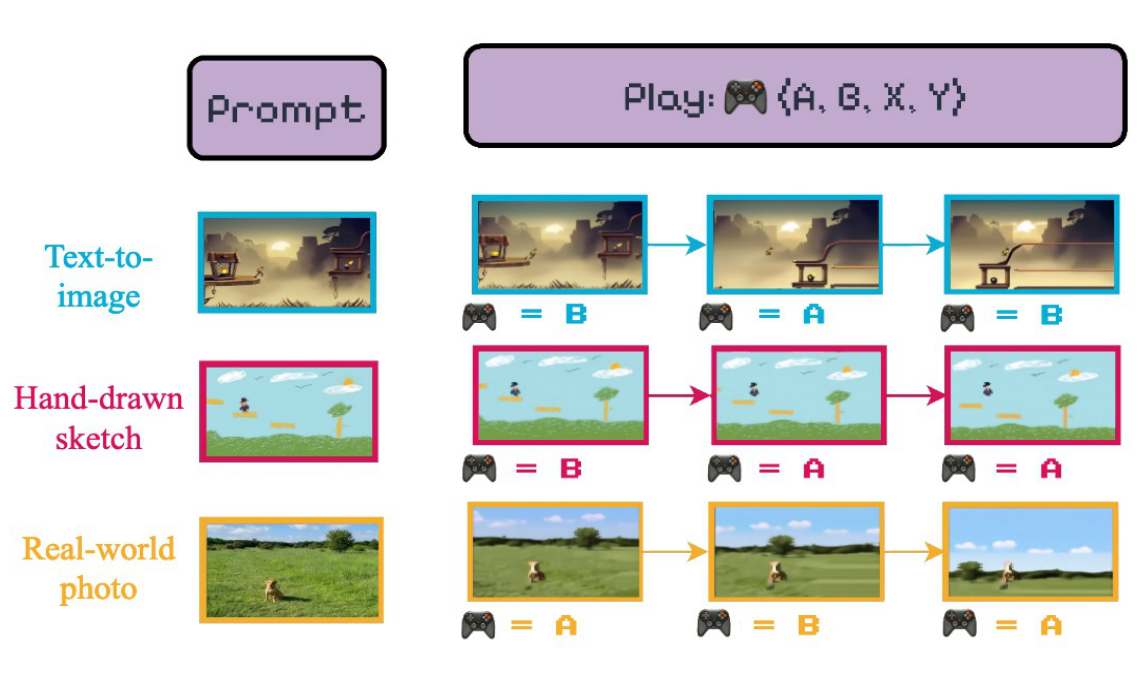
\includegraphics[width=0.85\linewidth,height=0.85\textheight,keepaspectratio]{images/video-generation/genie1_prompt_to_play_actions.png}\\[0.18em]
      {\scriptsize Source: CMU Lecture 26 \href{https://www.cs.cmu.edu/~mgormley/courses/10423/slides/lecture26-world-models.pdf}{World Models}}
    \column{0.47\textwidth}\footnotesize
      \textbf{Genie-1} is an interactive video\\generation model.\\[0.28em]
      \textbf{At test time:}
      \begin{itemize}\itemsep0.16em
        \item Takes a prompt (image) as input
        \item At each time step, accepts\\ an action given by the user
        \item Given the current frame \& action, generates the next frame
      \end{itemize}
      This simulates the style of interaction\\one would have with a video game.
  \end{columns}
\end{frame}

\begin{frame}[t]{2D Platformer Games (Setting)}
  \begin{columns}[T,onlytextwidth]
    \column{0.52\textwidth}
        \textbf{Q:} What is a 2D Platformer game?\\[0.5em]
        \textbf{A:} A 2D platformer is a video game where the player moves a character through a flat, two-dimensional world, usually by running, jumping, and avoiding obstacles or enemies. The gameplay often focuses on timing, movement precision, and reaching goals such as exits, items, or new areas.\\[0.8em]
        \textbf{Canonical Example:}\\
        Super Mario World for SNES
    \column{0.46\textwidth}
        \centering
        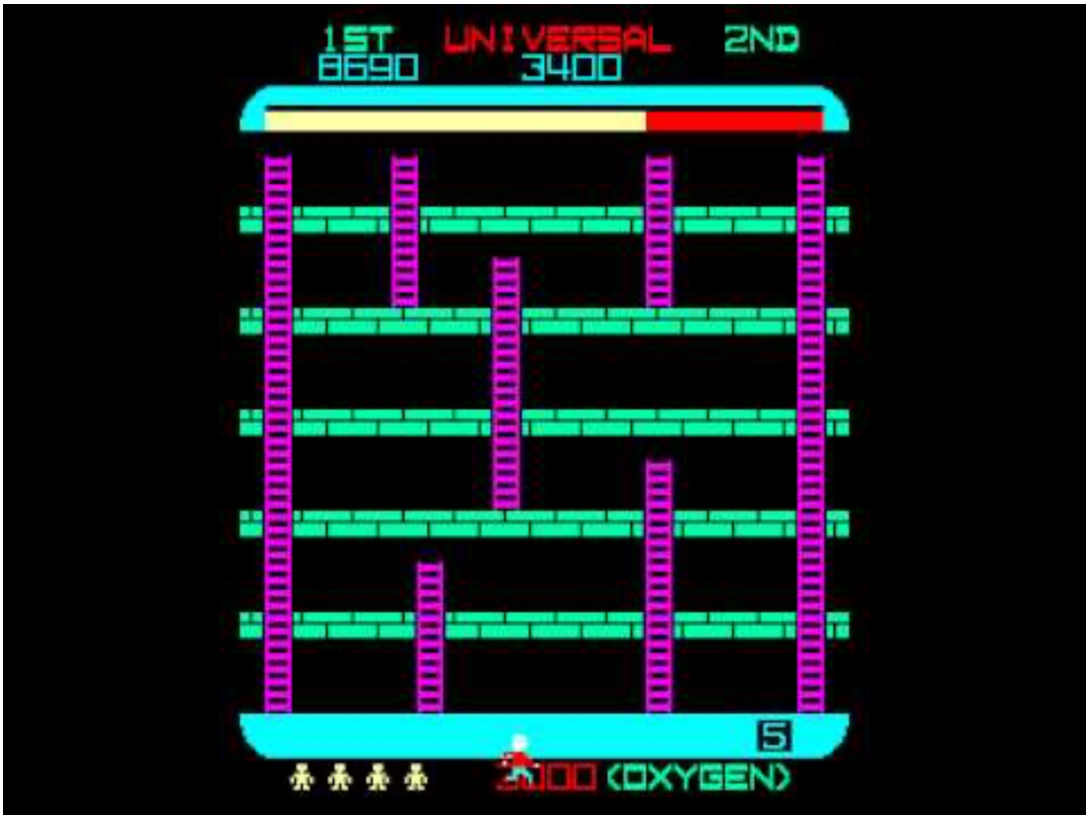
\includegraphics[width=0.98\linewidth,height=0.54\textheight,keepaspectratio]{images/video-generation/genie1_space_panic_first_2d_platformer.png}\\[-0.1em]
        {\scriptsize Space Panic: The first 2D platformer.\\
        Source: CMU 10-423, Lecture 26 (World Models); screenshot of \emph{Space Panic} (Universal, 1980).}
  \end{columns}
\end{frame}

\begin{frame}[t]{Genie-1: training data}
  \centering\vspace{0.06em}
  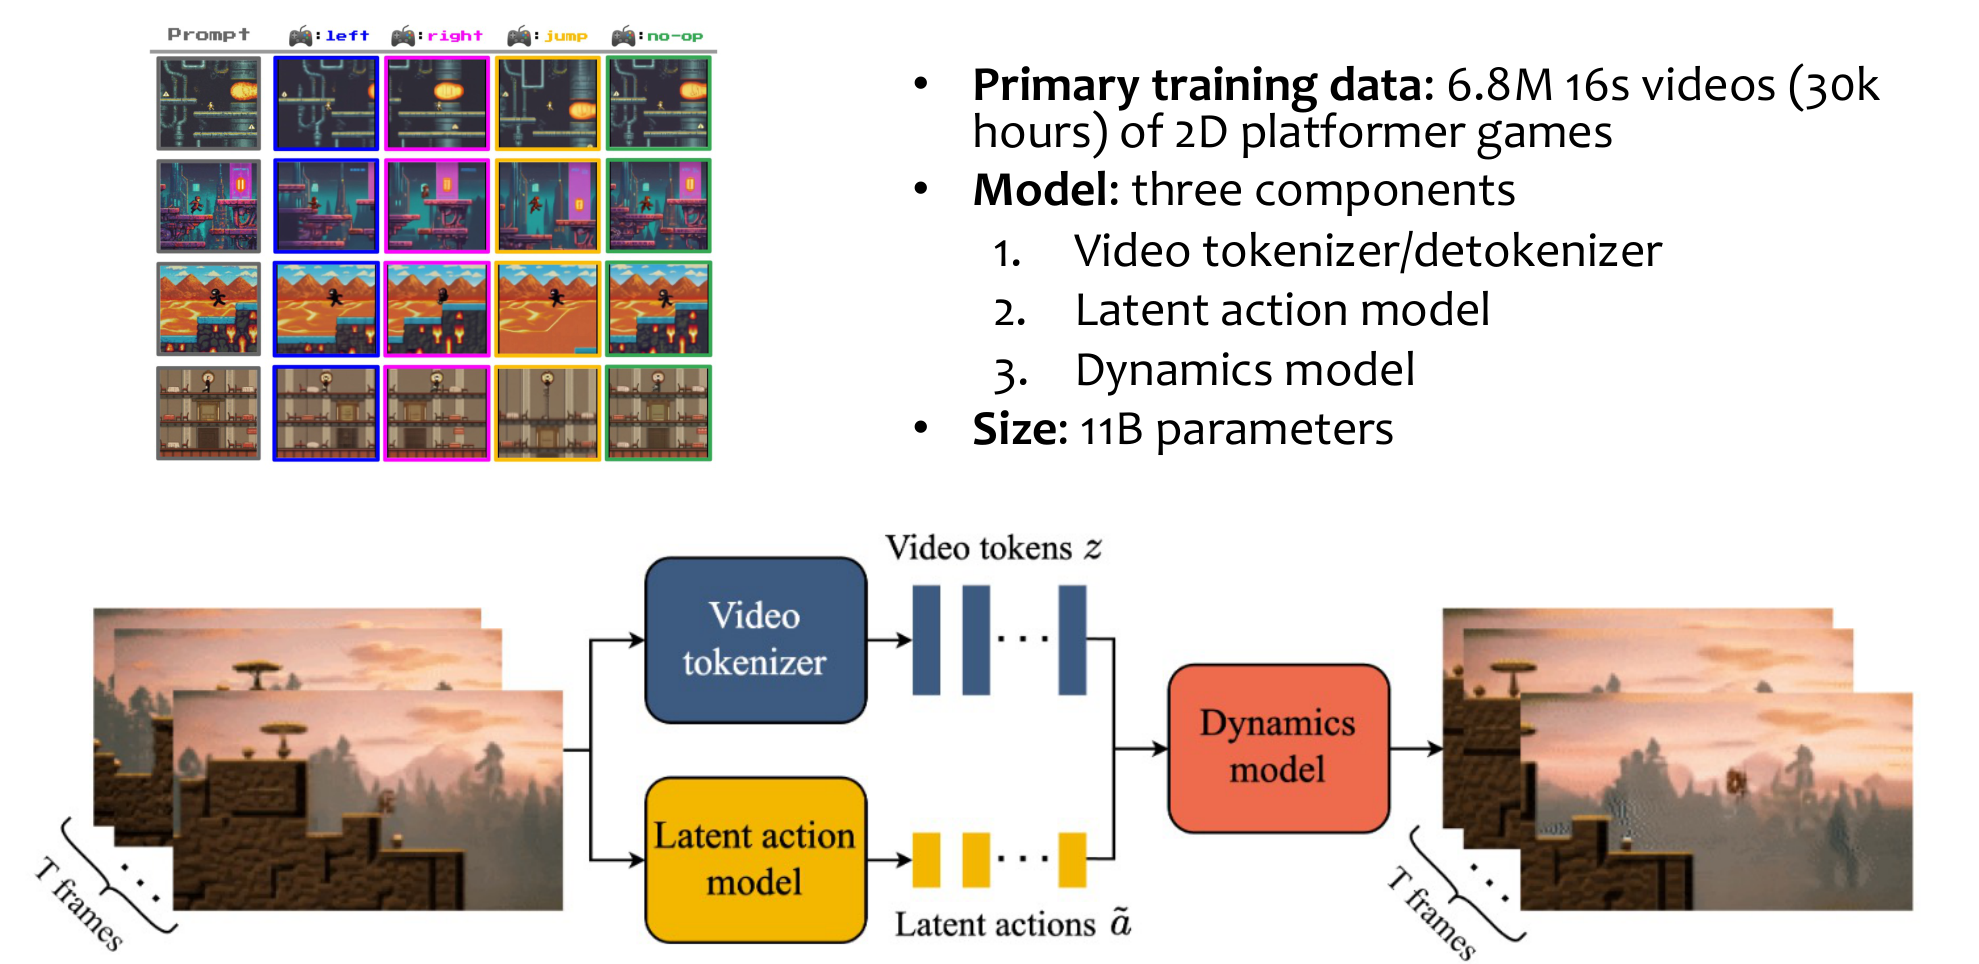
\includegraphics[width=\linewidth,height=0.86\textheight,keepaspectratio]{images/video-generation/genie1_training_data_components.png}\\[0.28em]
  {\scriptsize Source: CMU Lecture 26, World Models.}
\end{frame}

\begin{frame}[t]{Genie-1: video tokenizer}
  \centering\vspace{0.06em}
  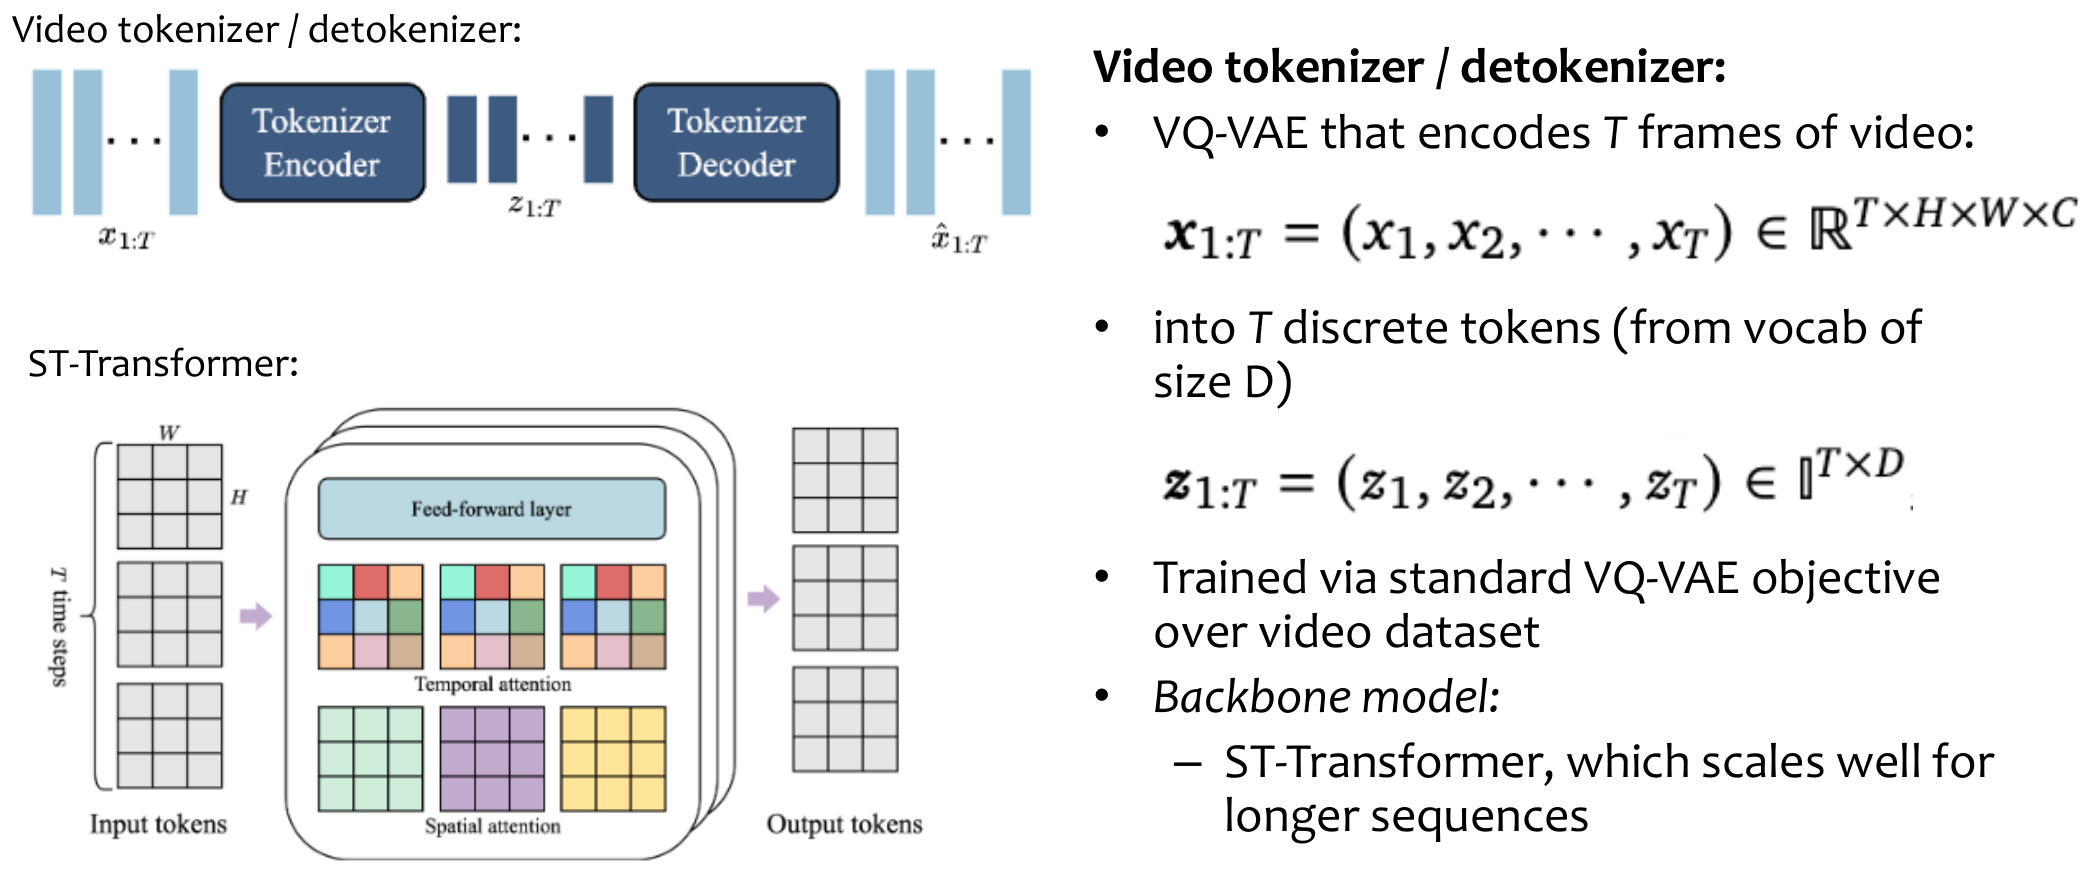
\includegraphics[width=\linewidth,height=0.86\textheight,keepaspectratio]{images/video-generation/genie1_video_tokenizer.png}\\[0.28em]
  {\scriptsize Source: CMU Lecture 26, World Models.}
\end{frame}

\begin{frame}[t]{Genie-1: latent action model}
  \centering\vspace{0.06em}
  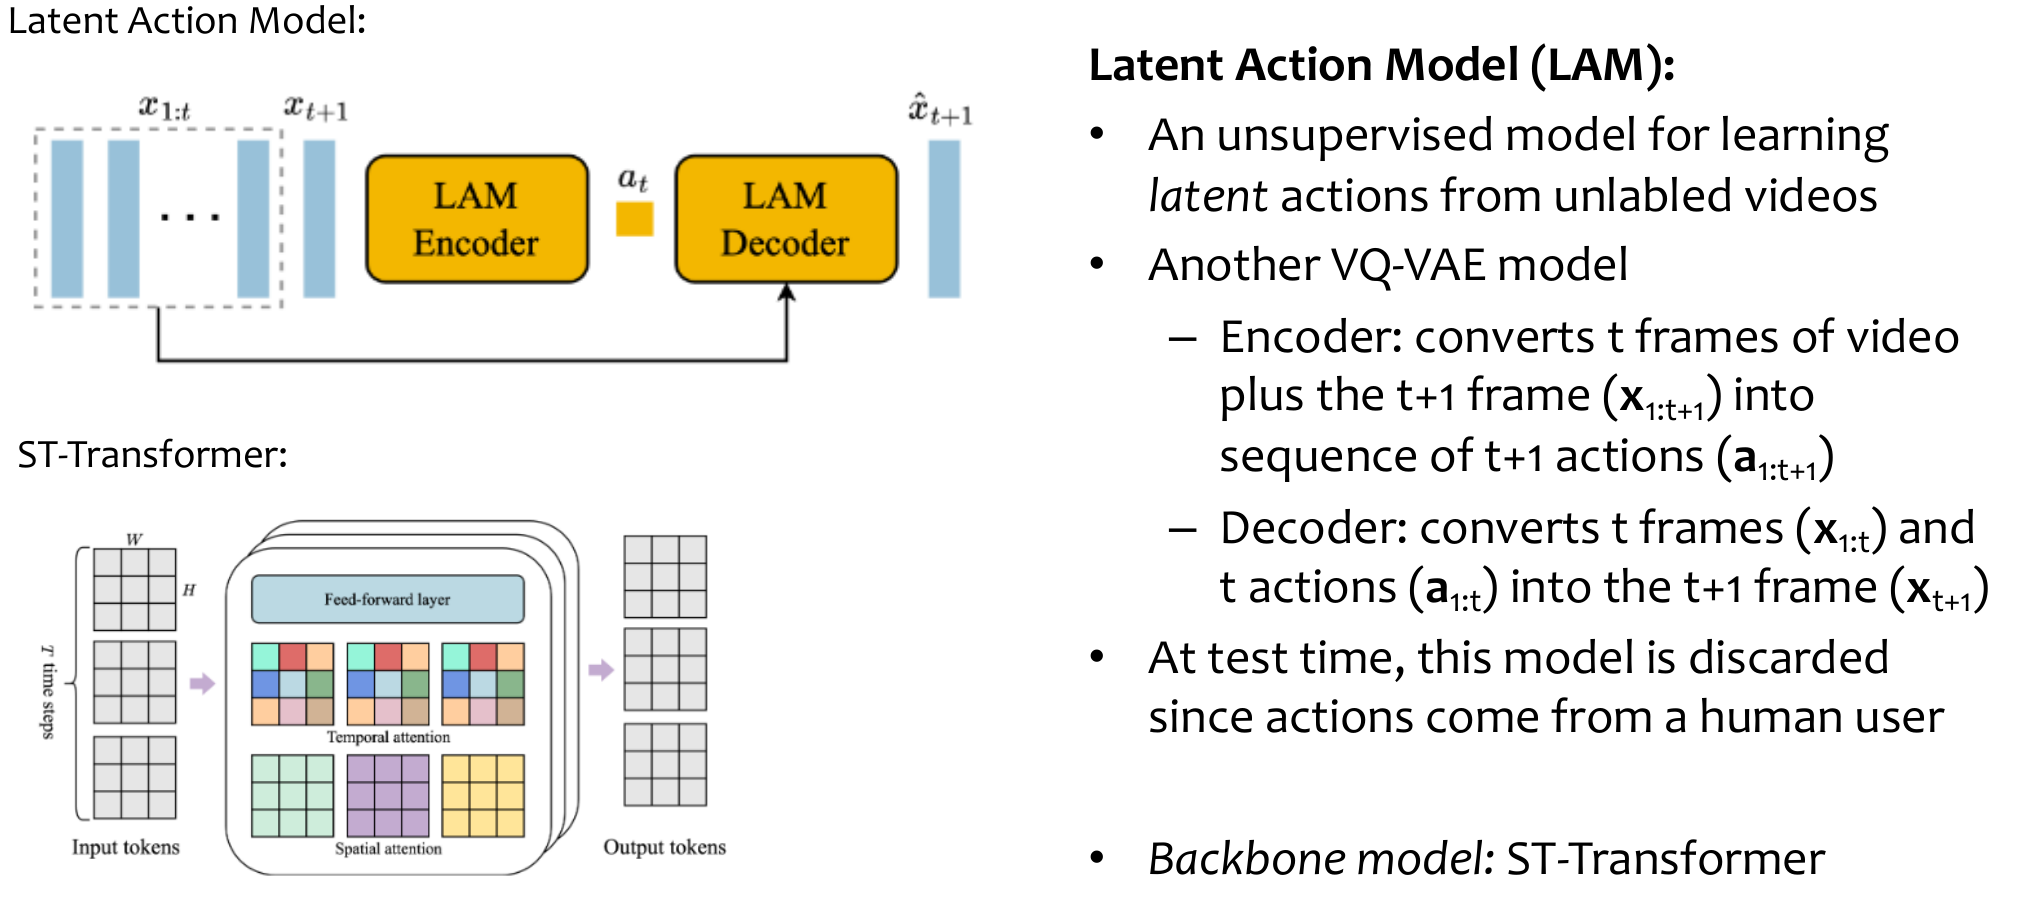
\includegraphics[width=\linewidth,height=0.86\textheight,keepaspectratio]{images/video-generation/genie1_latent_action_model.png}\\[0.28em]
  {\scriptsize Source: CMU Lecture 26, World Models.}
\end{frame}

\begin{frame}[t]{Genie-1: dynamics model (MaskGIT)}
  \centering\vspace{0.06em}
  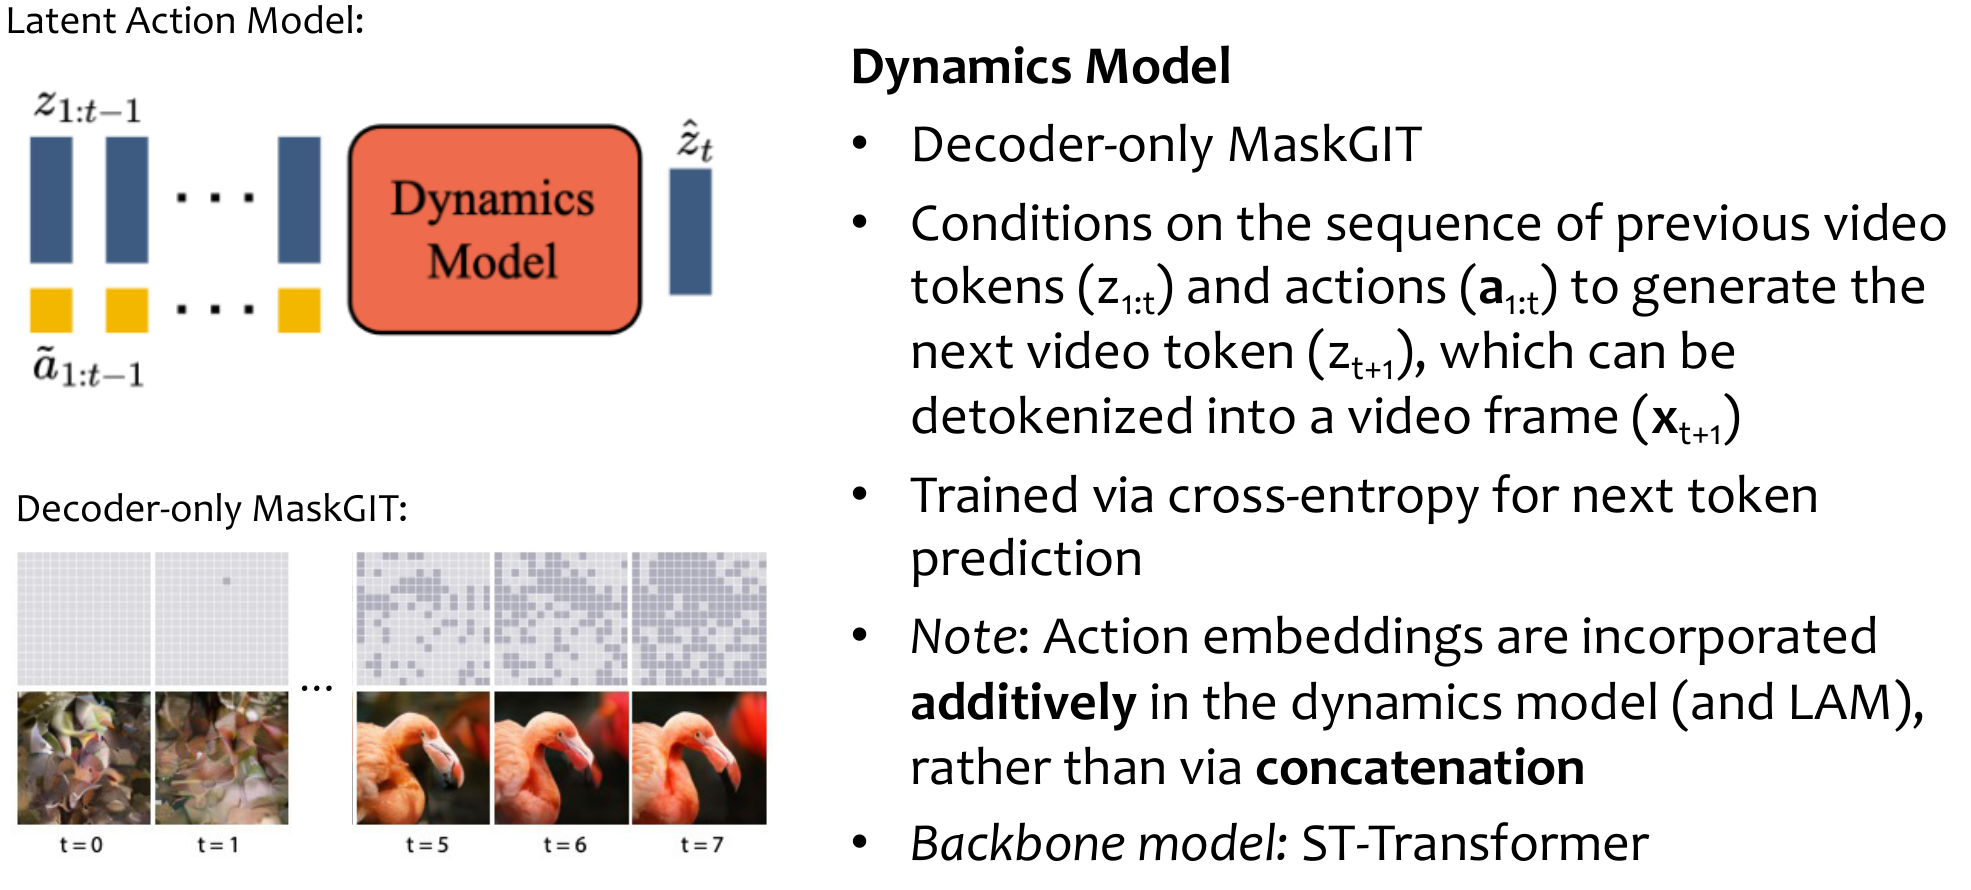
\includegraphics[width=\linewidth,height=0.86\textheight,keepaspectratio]{images/video-generation/genie1_dynamics_model_maskgit.png}\\[0.28em]
  {\scriptsize Source: CMU Lecture 26, World Models.}
\end{frame}

\begin{frame}[t]{Genie-1 at test time}
  \centering\vspace{0.06em}
  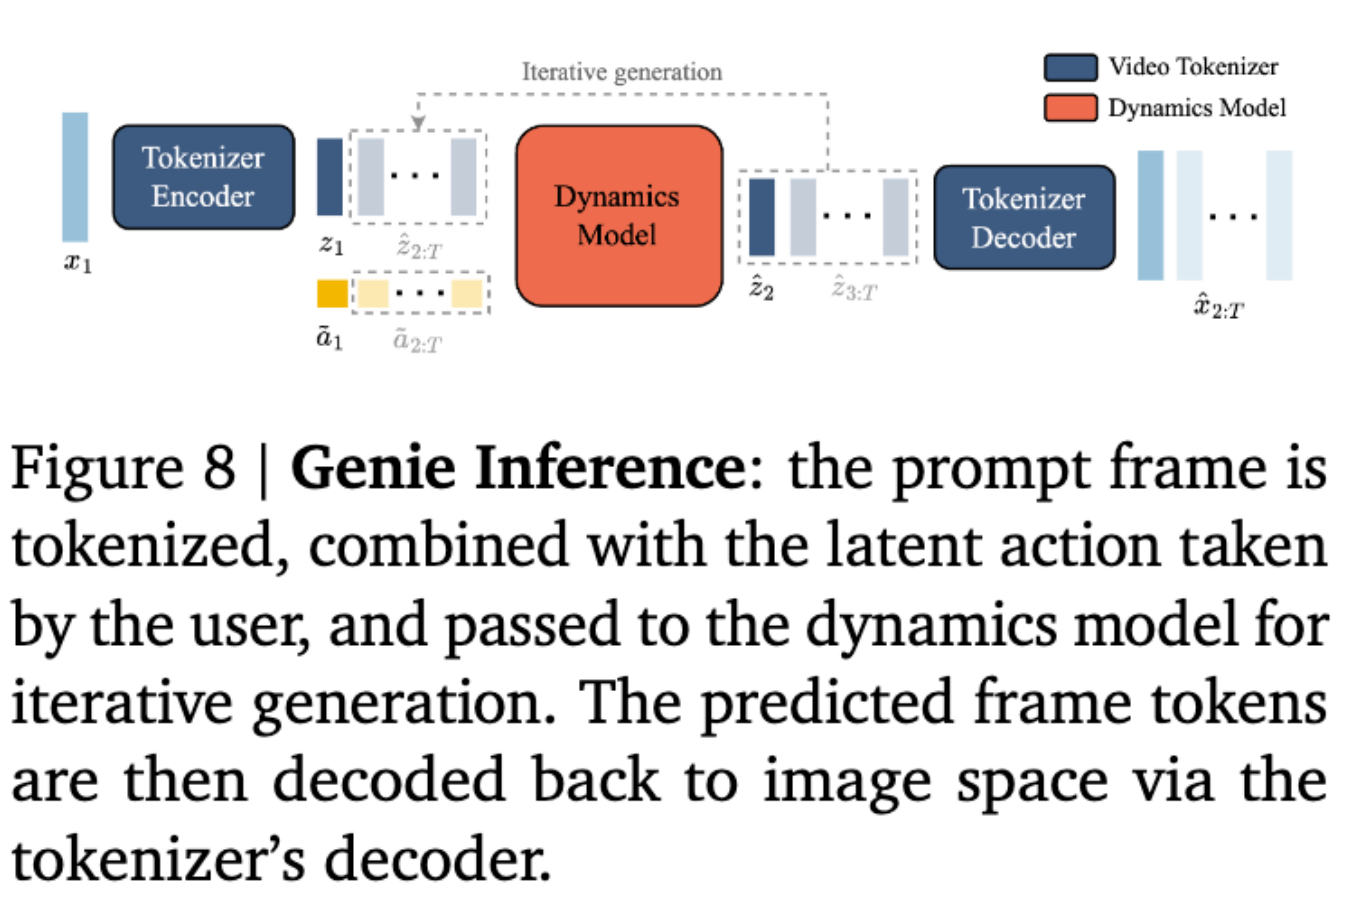
\includegraphics[width=\linewidth,height=0.86\textheight,keepaspectratio]{images/video-generation/genie1_inference_test_time.png}\\[0.28em]
  {\scriptsize Source: CMU Lecture 26, World Models.}
\end{frame}

\begin{frame}[t]{Genie-1 Qualitative Results}
  \begin{itemize}
    \item Images created with a text-to-image model can serve as a prompt.
    \item Then Genie-1 enables a user to interact directly with the environment.
    \item The latent actions are mapped to actual keys (a, s, d, f, etc.) so that the user can explore what they do.
  \end{itemize}
  \vfill
  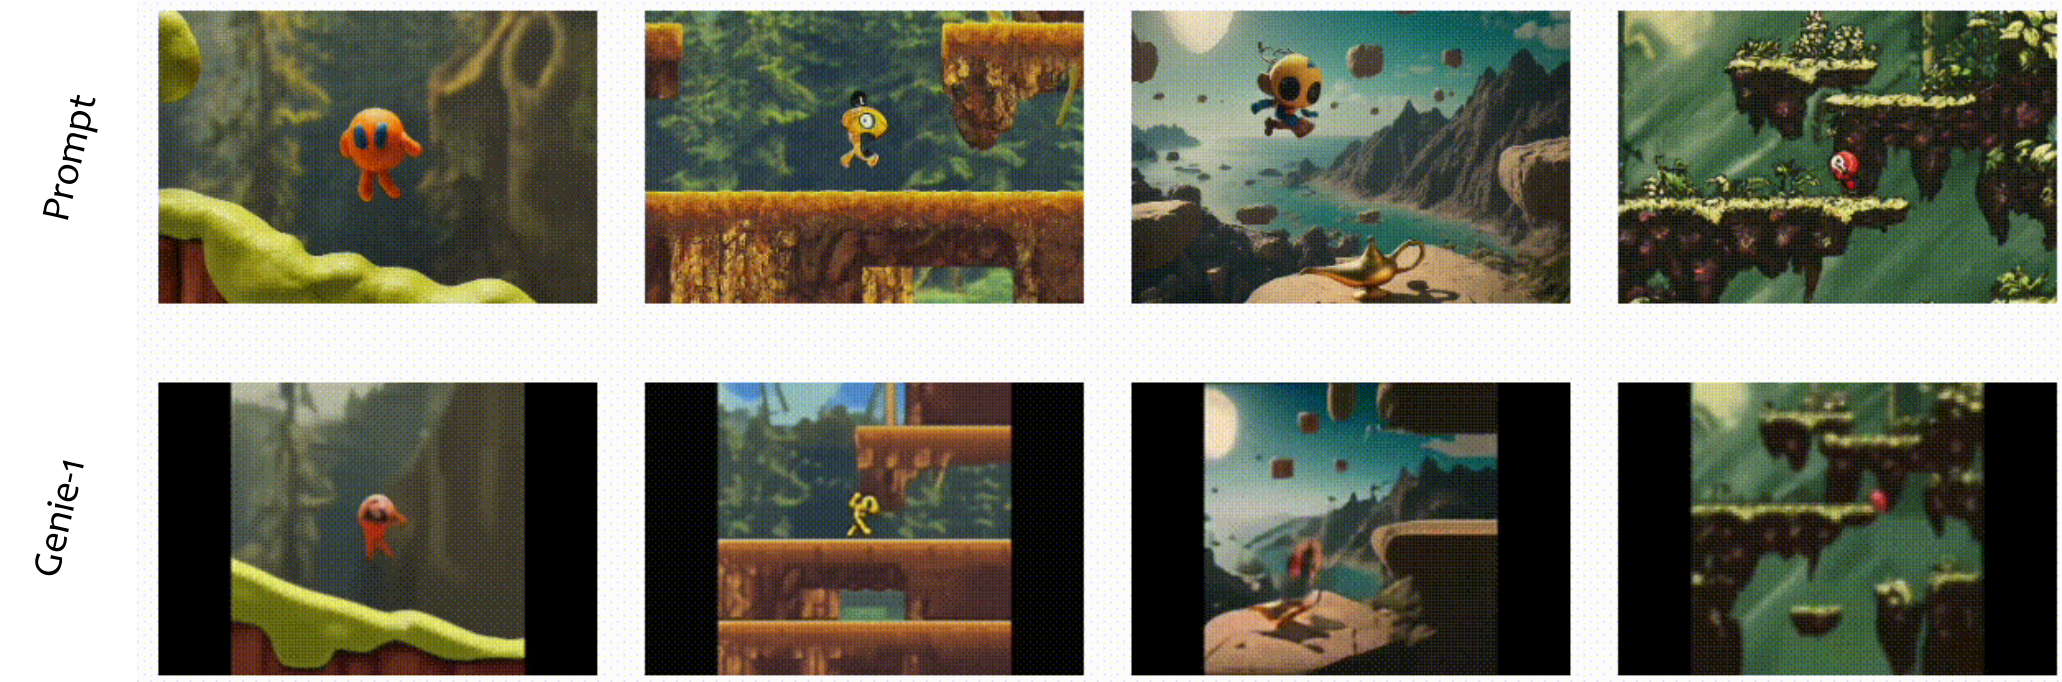
\includegraphics[width=0.85\linewidth,height=0.85\textheight,keepaspectratio]{images/video-generation/genie1_qualitative_results.png}\\[0.28em]
  {\scriptsize Source: CMU Lecture 26, World Models.}
\end{frame}

\begin{frame}[t]{Genie-1 Application to Robotics}
  \begin{columns}[T,onlytextwidth]
    \column{0.48\textwidth}
      \begin{itemize}\itemsep0.38em
        \item \textbf{Robotics dataset:}
        \begin{itemize}\itemsep0.2em
          \item 130k robotics demonstrations
          \item a simulation dataset (size unspecified)
          \item 209k episodes of real robot data
        \end{itemize}
        \item No actions included, just videos
      \end{itemize}
    \column{0.52\textwidth}
      \begin{itemize}\itemsep0.38em
        \item Training Genie on the robotics datasets learns a new model that can simulate ``game'' style play with a robotic arm as shown below
      \end{itemize}
  \end{columns}
  \vspace{0.6em}

  \begin{center}
    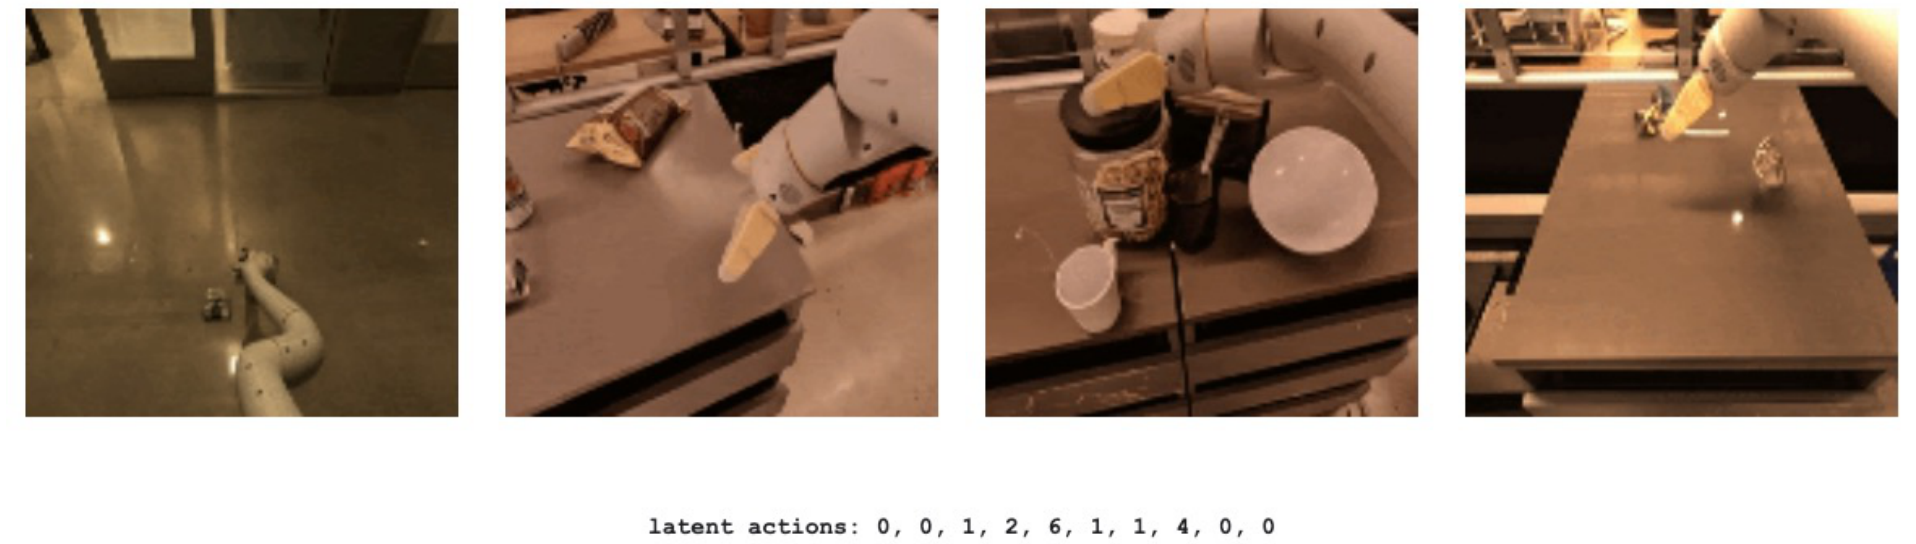
\includegraphics[width=0.76\linewidth,height=0.47\textheight,keepaspectratio]{images/video-generation/genie1_robotics_application.png}\\[0.28em]
    {\scriptsize Source: CMU Lecture 26, World Models.}
  \end{center}
\end{frame}

\begin{frame}[t]{Genie-1: Are the Latent Actions Transferable?}
  \begin{columns}[T,onlytextwidth]
    \column{0.52\textwidth}
      \begin{itemize}\itemsep0.45em
        \item CoinRun is a procedurally generated platformer.
        \item \textbf{Models:}
        \begin{enumerate}
          \item \textbf{Behavior Cloning:} train a policy given a dataset of each frame paired with the expert action (skyline)
          \item \textbf{Random Agent:} always take a random action (baseline)
          \item \textbf{LAM-based Policy:} train a policy given a dataset of each frame paired with the Genie latent action; separately learn a mapping from latent actions to expert actions from a few examples
        \end{enumerate}
      \end{itemize}
    \column{0.46\textwidth}
      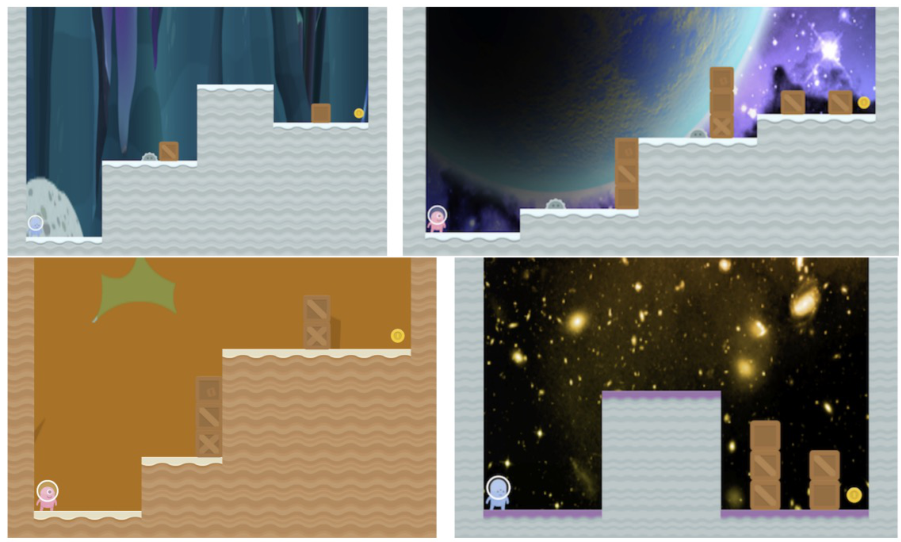
\includegraphics[width=\linewidth]{images/video-generation/genie1_coinrun_generated_levels.png}\\[0.15em]
      {\scriptsize Figure: Four generated CoinRun levels with the coin at the right.\\
      Source: CMU 10-423, Lecture 26 (World Models); CoinRun environment from Cobbe et al.,
      \href{https://arxiv.org/abs/1812.02341}{arXiv:1812.02341}.}
  \end{columns}
\end{frame}

\begin{frame}[t]{Genie-1: Are the Latent Actions Transferable? (Result)}
  \begin{columns}[T,onlytextwidth]
    \column{0.50\textwidth}
      \begin{itemize}\itemsep0.42em
        \item \textbf{Yes.} The LAM-based policy reaches the same score as the expert-action skyline (plotted as \emph{Oracle}) given as few as \textbf{200} action-labelled samples to fit the latent-to-real mapping, in both the easy and hard settings.
        \item Both stay far above the random agent.
        \item Metric: mean percentage of levels solved out of 100 samples, averaged over 5 seeds.
        \item So latent actions learned from unlabelled Internet video carry over to an environment the model never trained on, which is what makes them useful for control.
      \end{itemize}
    \column{0.48\textwidth}
      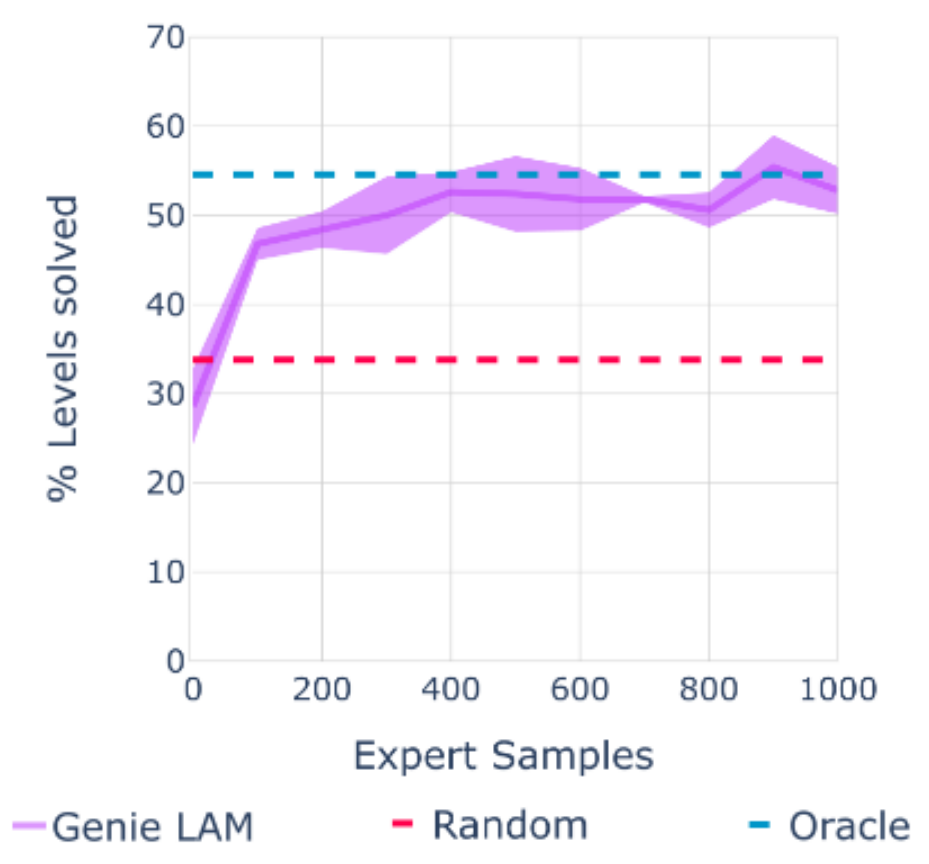
\includegraphics[width=0.9\linewidth,height=0.72\textheight,keepaspectratio]{images/video-generation/genie1_latent_action_transfer_plot.png}\\[0.28em]
      {\scriptsize Source: CMU Lecture 26, World Models; result per Bruce et al.\ (\href{https://arxiv.org/abs/2402.15391}{arXiv:2402.15391}), Fig.~15 (Easy).}
  \end{columns}
\end{frame}
